% 2009-10-22
\nr
\section{Kovalente Bindungen}

$1s^{2}2s^{2}2p^{2}\to1\overbrace{s^{2}\underbrace{2s2p_{x}2p_{y}2p_{z}}_{4\times sp^{3}}}^{\text{Hybridorbitale}}\to2p_{z}+3\times sp^{2}$

\begin{eqnarray*}
CH_{4}\\
\text{Methan}\end{eqnarray*}

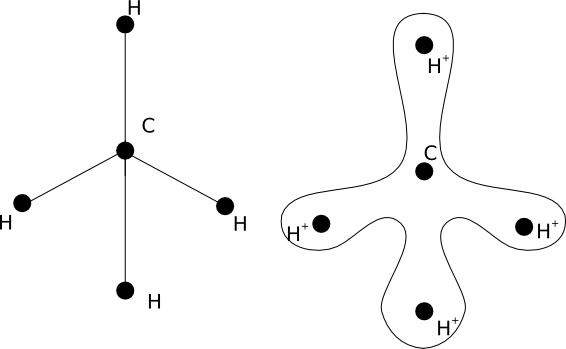
\includegraphics[scale=.5]{images/2009-10-27-hybridspiegelung.png}
FOLIEN
\subsection{Kristalle: $C$ (Diamant), $Si,\, Ge$}

$A^{III}B^{V}\to In\ Sb;\ Ga\ As$
\begin{labeling}{00.00.0000}
\item [{3D}] Graphit
\item [{2D}] Graphen (2004)
\item [{1D}] Kohlensotff-Nanoröhren (1991) 
\item [{0D}] Fulleren $\underbrace{C_{60}}_{\varnothing7,1\,\AA}$/$C_{70}$
(1985)
\end{labeling}

\subsection{Metallische Bindung}

Valenzelektronen sind delokalisiert

$\to$ Elektronengas

$Li$-Ionen: $r_{1}\sim0,6\,\AA$

$Li$-Kristall: $R_{0}\sim3\,\AA$

$\left.\dfrac{R_{0}}{r_{i}}\right|_{Cu}\sim1,33,\quad\left.\dfrac{R_{0}}{r_{i}}\right|\approx1,05$


\subsection{Wasserstoffbrückenbindung}

$\left.U_{i}\right|_{H}\sim13,6\,\text{eV};\quad\left.U_{i}\right|_{Na}\approx5,1\,\text{eV}$

$H\to$ Kovalente Bindung nur mit \underbar{einem} Nachbarn

$H_2 O$: GRAFIK

$HF^-_2$: GRAFIK

Wichtig f\"ur Organismus: DNA
Ammoniak: $NH_{3}$


\section{Struktur der Kristalle}

\underbar{Symmetrie:} Transformationen ,,unverändert{}`` erscheinen

Mathematik $\to$ Gruppentheorie
\begin{enumerate}
\item Punktgruppen (mindestens 1 Punkt ist fest)

\begin{enumerate}
\item z.\,B. Drehung um eine Drehachse GRAFIK, FOLIE
\item Spiegelung um eine Spiegelebene GRAFIK
\item Punktspiegelung GRAFIK
\end{enumerate}
\end{enumerate}
Spiegelung + Drehung

GRAFIK

Drehinversion

GRAFIK

\setcounter{enumi}{2} 
\begin{enumerate}
\item Raumgruppen (translative Symmetrieoperationen)
230 Gruppen Fedorov 
\begin{enumerate}
\item Gleitspiegelebene GRAFIK
\item Schraubung/Torsion GRAFIK
\end{enumerate}
\end{enumerate}
Kristallstruktur=Gitter+Basis

GRAFIK

$\underbrace{U(\vec{r})}_{\text{Umgebung}}=U(\vec{r}+\vec{R})$

$\vec{R}=n_{1}\vec{a}+n_{2}\vec{b}+n_{3}\vec{c},\;\vec{a},\vec{b},\vec{c}\text{ sind Baisvektoren}$

GRAFIK

Elementarzelle

primitive Elementarzelle $\rightarrow$ kleinstmögliche Elementrazelle 

(Abb.: primitive Elementarzellen)

\begin{tabular}{|c|c|c|}
\hline 
3D & Bravais- Gitter & Kristallstrukturen\tabularnewline
\hline
\hline 
Punktgruppen & 7 Kristallsysteme & 32\tabularnewline
\hline 
Raumgruppen & 14 Bravais- Gitter & 230 Raumgruppen\tabularnewline
\hline 
2D  & 5 & 17\tabularnewline
\hline
\end{tabular}

Bravais- Gitter (Basisobj. $\rightarrow$ Kugelsymmetrie) 

Kristallstruktur (beliebige Symmetrie)

(Abb.: Kristallstruktur= Gitter + Basis)

(Abb.: Rechtwinklige Kristallsysteme) 
